\documentclass{article}
\usepackage[utf8]{inputenc}
\usepackage{dashbox}
\usepackage{amsmath}
\usepackage{amssymb}
\usepackage{stackengine}
\usepackage{stmaryrd}
\usepackage{wasysym}
\usepackage[]{stix}
\usepackage{graphicx}
\usepackage{xcolor}

\newcommand{\BigAsterisk}{\mathop{\scalebox{3}{\raisebox{-0.2ex}{$\ast$}}}}%



\usepackage{parskip}
\usepackage[tmargin=1in,bmargin=1in,lmargin=0.75in,rmargin=0.75in]{geometry}

\usepackage{proof}

%\usepackage[most]{tcolorbox}

%\newtcbox{\dashedbox}[1][]{
%  math upper,
%  baseline=0.4\baselineskip,
%  equal height group=dashedbox,
%  nobeforeafter,
%  colback=white,
%  boxrule=0pt,
%  enhanced jigsaw,
%  boxsep=0pt,
%  top=2pt,
%  bottom=2pt,
%  left=2pt,
%  right=2pt,
%  borderline horizontal={0.5pt}{0pt}{dashed},
%  borderline vertical={0.5pt}{0pt}{dashed},
%  drop lifted shadow,
%  #1
%}


\newcommand{\einfer}[3]
        {\infer[(\textsc{#1})]{#3}{#2}}
\newcommand{\stacktwo}[2]{\stackanchor{\ensuremath{#1}}{\ensuremath{#2}}}
\newcommand{\stackthree}[3]{\stackanchor{\stacktwo{#1}{#2}}{\ensuremath{#3}}}
\newcommand{\stackfour}[4]{\stackanchor{\stackthree{#1}{#2}{#3}}{\ensuremath{#4}}}
\newcommand{\stackfive}[5]{\stackanchor{\stackfour{#1}{#2}{#3}{#4}}{\ensuremath{#5}}}
\newcommand{\stacksix}[6]{\stackanchor{\stackfive{#1}{#2}{#3}{#4}{#5}}{\ensuremath{#6}}}
\newcommand{\stackseven}[7]{\stackanchor{\stacksix{#1}{#2}{#3}{#4}{#5}{#6}}{\ensuremath{#7}}}

\newcommand\dboxed[1]{\dbox{\vphantom{t}\ensuremath{#1}}}

\newcommand{\hoare}[3]{\ensuremath{\{ #1 \}~ #2 ~\{ #3 \}}}
\newcommand{\viewshift}{\Rrightarrow}
\newcommand{\viewshiftBack}{\Lleftarrow}
\newcommand{\unit}{\epsilon}
\newcommand{\true}{\textsf{True}}
\newcommand{\false}{\textsf{False}}
\newcommand{\bool}{\textsf{bool}}
\DeclareMathOperator{\rel}{rel}
\DeclareMathOperator{\TPCM}{TPCM}
\DeclareMathOperator{\MonoidBase}{MonoidBase}
\DeclareMathOperator{\MonoidExt}{MonoidExt}
\DeclareMathOperator{\Frac}{Frac}
\newcommand{\monoid}[1]{\textsf{monoid}~#1}
\renewcommand{\eqdef}{\triangleq}
\newcommand{\borrow}[2]{\textsc{\&}^{#1}#2}
\newcommand{\pointsto}{\hookrightarrow}

%\DeclareFontEncoding{LS1}{}{}
%\DeclareFontSubstitution{LS1}{stix}{m}{n}
%\DeclareSymbolFont{arrows2}       {LS1}{stixsf}   {m}{it}
%\SetSymbolFont{arrows2}     {bold}{LS1}{stixsf}   {b}{it}
%\DeclareSymbolFontAlphabet{\mathsfit}{arrows2}
%\DeclareMathSymbol{\rightarrowgtr}{\mathrel}{arrows2}{"5F}

\newcommand{\refines}{\rightarrowgtr}

\newcommand{\ltIntersect}{\sqcap}
\newcommand{\ltLe}{\sqsubseteq}
\newcommand{\ltGe}{\sqsupseteq}
\DeclareMathOperator{\lifetime}{lifetime}
\DeclareMathOperator{\borrowed}{borrowed}

\newcommand\Bigcircle{\raisebox{-0.5mm}{\scalebox{1.7}{$\bigcirc$}}}


\let\active\undefined
\DeclareMathOperator{\active}{active}



%\newcommand{\shardProduct}{\rtimes}
%\newcommand{\shardProduct}{\rightmoon}
%\newcommand{\shardProduct}{\rsub}
\newcommand{\shardProduct}{\ogreaterthan}

\begin{document}

Here, we describe a PCM-based program logic for reasoning about concurrent programs,
with a built-in notion of ``PCM refinement'' to provide modularity that is both useful in its own right
and particularly useful for reasoning about ``read-only'' state.

\textbf{Monoid definitions}

%We write $\widehat{M} = (M, \cdot, \mapsto)$ is a Partial Commuative Monoid (PCM) if,
%where $\cdot : M \times M \to M^?, \text{~~comm., assoc.}$
%and $\mapsto : M \times M \to \bool, \text{~~trans., refl., monotonic}$,
%we have
%\begin{align*}
%& a \cdot b = b \cdot a & & \text{(commutativity)}\\
%& (a \cdot b) \cdot c = a \cdot (b \cdot c) & & \text{(associativity)}\\
%& (a \mapsto b) \land (b \mapsto c) \implies a \mapsto c && \text{(transitivity)}\\
%& (a \mapsto a) && \text{(reflexitivity)}\\
%& (a \mapsto b \land a \cdot c \ne \bot \implies b \cdot c \ne \bot \land a \cdot c \mapsto b %\cdot c) && \text{(monotonic)}
%\end{align*}


%\\
%Monoid $\mathcal{M} := M ~|~ \mathcal{M}\otimes\mathcal{M} ~|~ E[\mathcal{M}]$\\
%\\
%\textbf{Base monoid} $M$ equip with $\cdot$ commutative, associative,
%unit $\unit \in M$, bot element $\bot \in M$, and
%$a \mapsto_M b \eqdef (\forall c .~ a\cdot c \ne \bot \implies b\cdot c \ne \bot)$\\
%\\
%\textbf{Product monoid} $M \otimes N$ where $(a\otimes b)\cdot(c \otimes d) = (a\cdot c)\otimes(b\cdot d)$
%and $(a\otimes b) \mapsto (a' \otimes b') \eqdef (a \mapsto a') \land (b \mapsto b')$\\
%\\
%\textbf{Extension monoid} $E[M]$. Monoid $E,\cdot$, predicate $\rel : E \times M \to \bool$,
%and $b \mapsto b' \eqdef
%(\forall p, q .~ \rel(b \cdot p, q) \implies \exists b' .~ \rel(b' \cdot p, q') \land (q \mapsto q'))$
%and
%$\forall b, a, a' .~ \rel(b,a) \land \rel(b,a') \implies a \mapsto a'$\\
%\\
%\\
%Define $\le$ by $a \le b \eqdef \exists b . a \cdot c = b$.\\
%\\

We start by defining what it means to be a PCM with a transition relation $\mapsto$.
We call this a \emph{Transitional PCM} (TPCM).

Let $\widehat{M} = (M, \cdot, \mapsto)$ where
where $\cdot : M \times M \to M^?$
and $\mapsto : M \times M \to \bool$.
(We use $M^? \eqdef M \cup \{\bot\}$.)

We say that $\mapsto$ is \emph{monotonic} if
\[ \forall a, b, c.~ (a \mapsto b) \land (a \cdot c \ne \bot) \implies (b \cdot c \ne \bot) \land (a \cdot c \mapsto b \cdot c) \]
This allows us to define what it means to be a TPCM,
\[
  \einfer{TPCM}{
    \stackthree{
      \widehat{M} = (M, \cdot, \mapsto)
    }{
      \cdot : M \times M \to M^?, \text{~~comm., assoc.}
    }{
      \mapsto : M \times M \to \bool, \text{~~trans., refl., monotonic}
    }
  }{
    \TPCM(\widehat{M})
  }
\]
Note that we can always construct a TPCM by picking $\cdot$ to be commutative and associative,
and then by definition setting $\mapsto$ to be,
\[
  a \mapsto b = \forall c .~ a \cdot c \ne \bot \implies b \cdot c \ne \bot
\]
However, we can also set $\mapsto$ to be more restrictive, which will be useful later.

\textbf{TPCM Example}

Consider a \emph{Sharded State Machine} (SSM). (This is similar to the STS common in the literature but framed a little differently.)

An SSM is given by \textbf{(i)} some PCM state $S, \cdot$, \textbf{(ii)} an invariant $inv : S \to \bool$ and a sharded transition $\rightsquigarrow : S \times S \to \bool$. For a sharded state
machine, the invariant inductivity predicate is given by,
\[
  inv(a \cdot c) \land (a \rightsquigarrow b) \implies inv(b \cdot c)
\]
(Note: $\rightsquigarrow$ is neither transitive nor required to be monotonic here. However, an alternative definition would require $\rightsquigarrow$ to be monotonic, in which case we could
simplify the inductivity predicate to $inv(a) \land (a \rightsquigarrow b) \implies inv(b)$.)

We can define a TPCM to correspond to this SSM by,
\[M \eqdef \{m \in S : \exists c .~ inv(m \cdot c) \}\]
\[a \cdot_M b \eqdef 
  \begin{cases}
      a \cdot b & \text{if } a \cdot b \in M\\
      \bot,              & \text{otherwise}
  \end{cases}\]
and finally we can define $\mapsto$ as the transitive closure of $\mapsto_\text{pre}$ defined as,
\[
a \mapsto_{\text{pre}} b \eqdef
  \exists a_0, b_0, c .~ (a = a_0 \cdot c) \land (b = b_0 \cdot c) \land a_0 \rightsquigarrow b_0
\]

\textbf{TPCM refinements (motivation)}

There are a handful of reasons to want to modularize PCM definitions:
\begin{itemize}
  \item The ``base language'' may provide some ``points to'' assertion $\ell \pointsto v$,
    and then the user wants to build something else on top of that (like a fractional permission logic or similar) without needing to inject it into the native definition.
  \item You have some PCM $N$ (custom built for your application), and you want to build a reader-writer lock to manage
    access to the state of $N$, without encoding the reader-writer lock protocol into $N$.
  \item You have some PCM $N$, and you want to manage part of it via some hash table implementation. You want to verify the hash table implementation independently (e.g., via some SSM strategy) and then use it modularly to manage some part of the $N$-state.
  \item You have some PCM $N$ with a counter field, and you want to write the counter-manipulation code as its own independent module.
\end{itemize}
These are all things that have come up in VeriBetrKV.

We'll develop the concept of a TPCM refinement, denoted $\widehat{M} \refines \widehat{N}$.
In a modular design, $\widehat{M}$ will be the ``sub-component'', while $\widehat{N}$
is the client.

For example, a hypothetical cache architecture might have a ``main'' ghost state \textsf{Cache}
represented as an SSM.
We might have a sub-component $\textsf{RwLock} \refines \textsf{Cache}$,
another sub-component $\textsf{HashTable} \refines \textsf{Cache}$,
and even further a sub-component $\textsf{Counter} \refines \textsf{HashTable}$.

\begin{center}
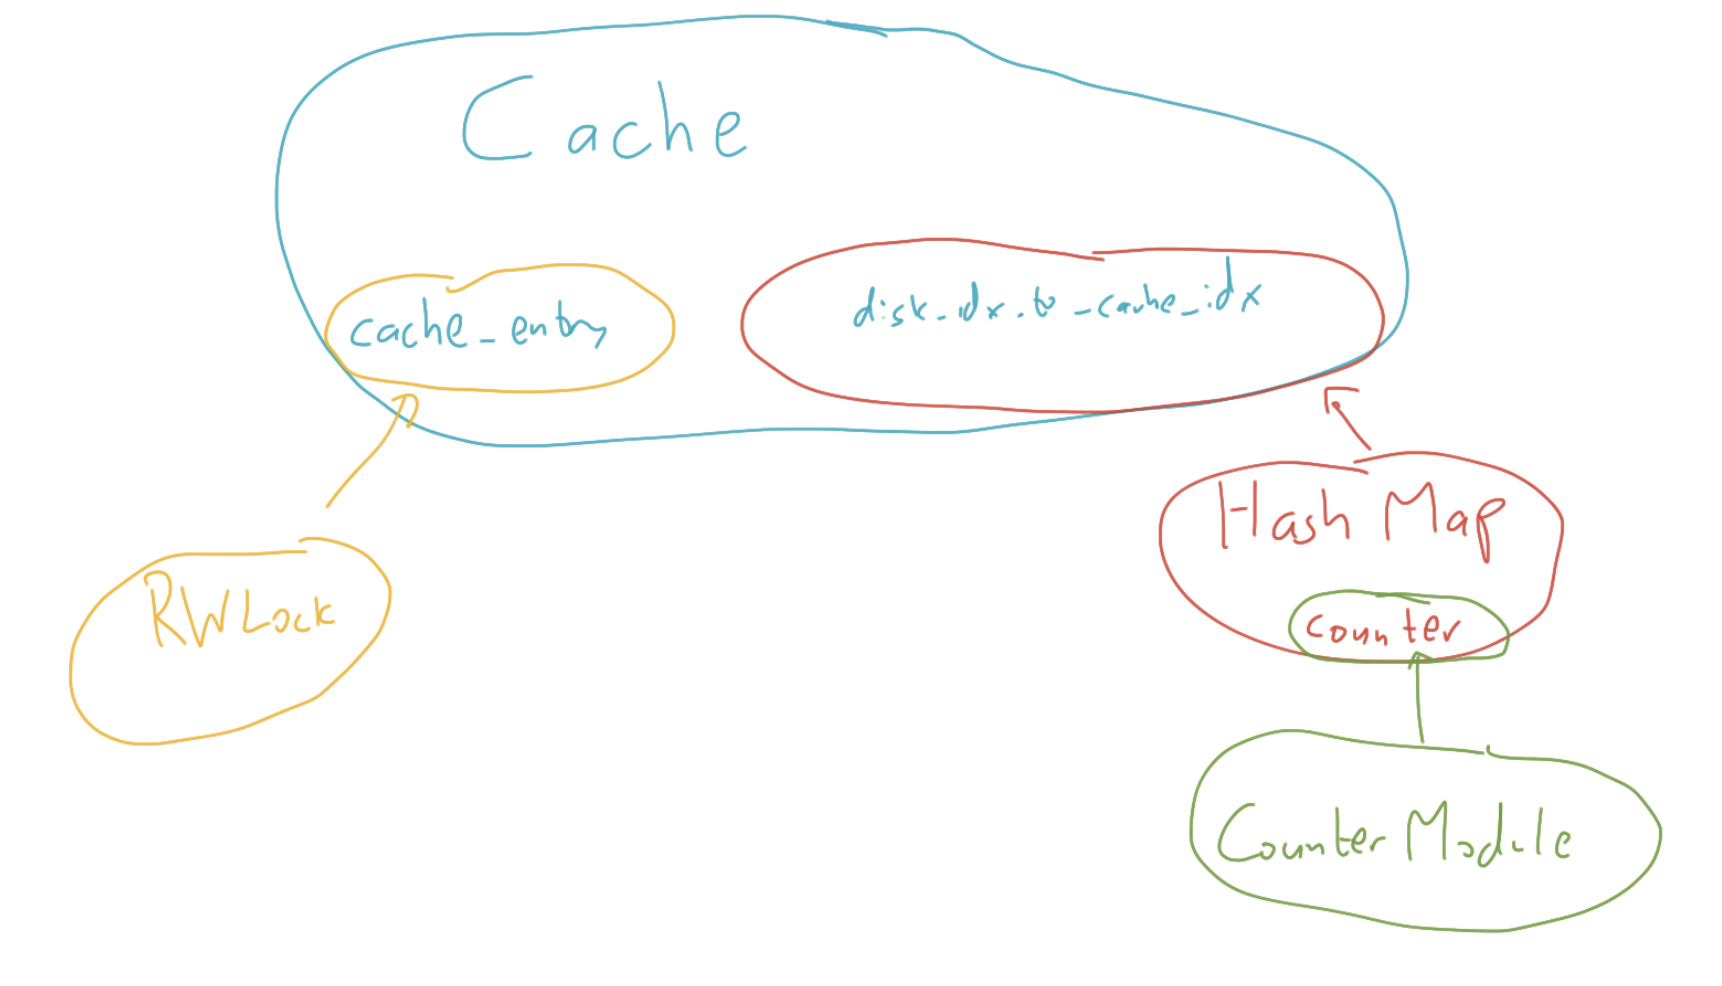
\includegraphics[scale=0.3]{hypothetical-cache-architecture.png}
\end{center}

\textbf{TPCM refinements}

We'll use the symbol $\refines$ to denote refinement. Yeah, you can tell I scoured the \LaTeX~ documentation for this thing, but I actually like it: it suggests that the thing on the left is more ``broken up'' (e.g., like in a fractional logic).

We use $\widehat{M} \refines_{\rel} \widehat{N}$ to denote that $\widehat{M}$ \emph{refines} $\widehat{N}$ via a relation $\rel : M \times N \to bool$. Of course, it must satisfy some conditions 
(and this is why we allow for flexibility in the definition of $\mapsto$ above).

\[
  \einfer{TPCM-Refinement}{
    \stackfive{
      \TPCM(\widehat{M}) \quad \TPCM(\widehat{N})
    }{
      \rel : M \times N \to \bool
    }{
      \rel(\unit, \unit)
    }{
       (\forall b, b', q .~ b \mapsto b' \land \rel(b, q) \implies \exists q' .~ \rel(b', q') \land (q \mapsto q'))
    }{
      \forall b, a, a' .~ \rel(b,a) \land \rel(b,a') \implies a \mapsto a'
    }
  }{
    \widehat{M} \refines_{\rel} \widehat{N}
  }
\]

\textbf{Using ghost state in programs}

We instantiate instances of monoidal ghost state at \emph{locations}.
The notation $\dboxed{a}^\gamma$ means that state $a$ is at location $\gamma$.
Typically, locations are considered arbitrary values; here, we have to do a little
more to handle the relationships between different ghost states.

For example, suppose we have a refinement $\widehat{M} \refines_{\rel} \widehat{N}$.
Perhaps $\widehat{M}$ represents a reader-writer protocol or something similar.
Furthermore, let's say we're tracking ghost state $n \in N$ at location $\gamma$:
we will use the notation $\dboxed{n}^\gamma$.

Now, we want to use the $\widehat{M}$ protocol to help manage that state.
We'll need some rules for ``exchanging'' the $\widehat{M}$-state with $\widehat{N}$-state.
Furthermore, when we manage the $\widehat{M}$-state, we'll need to somehow ``remember''
that it corresponds to the $\widehat{N}$-state at $\gamma$, via the refinement $\rel$.
We will track this information in the location value.

Thus, we'll define the location values recursively, reusing the $\refines$ notation:

$\gamma ~~:=~~ \alpha ~~|~~ \alpha \refines_{\rel} \gamma$.

Here, $\alpha$ denotes any ``base location.'' We will define rules that let us
convert $\dboxed{n}^\gamma$ state to and from $\dboxed{m}^{\alpha \refines_{\rel} \gamma}$
state.

Here are our rules for manipulating TPCM ghost state, which are mostly standard except
the ones involving $\refines$.

\[
  \true \implies \dboxed{\unit}^\gamma
\]

\[
  \dboxed{\bot}^\gamma \implies \false
\]

\[
  \dboxed{t\cdot u}^\gamma\iff\dboxed{t}^\gamma * \dboxed{u}^\gamma
\]

\[
  \einfer{Ghost-Alloc}{
    \TPCM(\widehat{M}) \quad a\in M
  }{
    \true \viewshift \exists\alpha.~ \dboxed{a}^\alpha
  }
\]

\[
  \einfer{Ghost-Refinement-Alloc}{
    \stacktwo{
      \widehat{M} \refines_{\rel} \widehat{N}
    }{
      \rel(m, n)
    }
  }{
    \dboxed{n}^\gamma \viewshift \exists \alpha.~ \dboxed{m}^{\alpha \refines_{\rel} \gamma}
  }
\]

\[
  \einfer{Ghost-ViewShift}{
    a \mapsto b
  }{
    \dboxed{a}^\gamma \viewshift \dboxed{b}^\gamma
  }
\]

\[
  \einfer{Ghost-Refinement-Exchange}{
    \stacktwo{
      \widehat{M} \refines_{\rel} \widehat{N}
    }{
      \forall p,q.~ \rel(b\cdot p) = Some(q) \implies \exists q' .~ \rel(b' \cdot p) = Some(q') \land (a \cdot q \mapsto a' \cdot q')
    }
  }{
    \dboxed{b}^{\alpha \refines_{\rel} \gamma} * \dboxed{a}^\gamma
      \viewshift
    \dboxed{b'}^{\alpha \refines_{\rel} \gamma} * \dboxed{a'}^\gamma
  }
\]

\textbf{Justification.}

To justify these rules, we can roll up all the $\dboxed{m}^\gamma$ values into a mega-monoid (or resource algebra)
one defined as a mapping from locations to monoid elements.
Then we show that all those rules above follow from frame-preserving updates.

\textbf{Notes about abstraction.}

When using a refinement
$\widehat{M} \refines \widehat{N}$
to abstract out some subcomponent, we observe that $\widehat{M}$ (which corresponds to the subcomponent) needs to be defined with respect to the base state $\widehat{N}$,
which initially seems a little strange. Shouldn't we define the subcomponent \emph{first}, and then build the larger components out of those?

And yes, if for example $\widehat{M}$ is a reader-writer lock, then $\widehat{M}$ and the refinement $\rel$ will need to be defined in terms of $\widehat{N}$. However, this is not really so different than using a templated type, e.g., writing \texttt{RwLock<T>} to create a mutex storing type \texttt{T}.

\textbf{Borrows and read-only state.}

I think we can use a fairly simple system for representing (shared) borrows. 
We use $\kappa$ to represent a lifetime variable.
$\borrow{\kappa}{A}$ represents some borrowed proposition;
$\active(\kappa)$ indicates that lifetime $\kappa$ is active,
and $\borrowed(\kappa, A)$ indicates you can get back exclusive access to $A$
once the lifetime $\kappa$ expires.

We use $\kappa_1 \ltIntersect \kappa_2$ to represent lifetime intersection
and $\kappa_1 \ltLe \kappa_2$ to represent lifetime inclusion.

Of course, the intent is that the verification framework will use some sort of borrow-checker
to identify the lifetimes and perform these automatically.

(Note: RustBelt uses a much more complex system - need to understand why; am I missing something or is it for some feature I don't need?)

\[
  \einfer{Borrow-begin}{
  }{
    A \viewshift \exists
        \kappa .~ \active(\kappa) * \borrowed(\kappa, A) * \borrow{\kappa}{A}
  }
\]

\[
  \einfer{Borrow-end}{
  }{
    \active(\kappa) * \borrowed(\kappa, A) \viewshift A
  }
\]

\[
  \einfer{Borrow-dupe}{
  }{
    \borrow{\kappa}{A} \viewshift \borrow{\kappa}{A} * \borrow{\kappa}{A}
  }
\]

\[
  \einfer{Reborrow}{
    \kappa_1 \ltGe \kappa_2
  }{
    \borrow{\kappa_1}{A} \viewshift \borrow{\kappa_2}{A}
  }
\]

\[
  \active(\kappa_1 \ltIntersect \kappa_2) \iff \active(\kappa_1) * \active(\kappa_2)
\]

Next, let's add some rules for making use of borrowed TPCM state.

\[
  \true \implies \borrow{\kappa}{\dboxed{\unit}^\gamma}
\]

\[
  \active(\kappa) * \borrow{\kappa}{\dboxed{\bot}^\gamma} \implies \false
\]

\[
  \einfer{Borrow-Combine}{
    \forall r .~ m \le r \land n \le r \implies k \le r
  }{
    \borrow{\kappa}{\dboxed{m}^\gamma} * \borrow{\kappa}{\dboxed{n}^\gamma} \viewshift \borrow{\kappa}{\dboxed{k}^\gamma}
  }
\]

\[
  \einfer{Borrow-Ghost-ViewShift}{
    c \cdot a \mapsto c \cdot b
  }{
    \active(\kappa) * \borrow{\kappa}{\dboxed{c}^\gamma} * \dboxed{a}^\gamma
    \viewshift
    \active(\kappa) * \dboxed{b}^\gamma
  }
\]

Finally, rules to allow borrows to interact with TPCM refinements:

\[
  \einfer{Borrow-Back}{
    \stacktwo{
      \widehat{M} \refines_{\rel} \widehat{N}
    }{
      \forall p, b .~ \rel(m \cdot p, b) \implies a \le b
    }
  }{
    \borrow{\kappa}{\dboxed{m}^{\delta \refines \gamma}} \viewshift \borrow{\kappa}{\dboxed{a}^\gamma}
  }
\]

\[
  \einfer{Borrow-Ghost-Refinement-Exchange}{
    \stacktwo{
      \widehat{M} \refines_{\rel} \widehat{N}
    }{
      \forall p,q.~ \rel(c\cdot b\cdot p, q) \implies \exists q' .~ \rel(c \cdot b' \cdot p, q') \land (a \cdot q \mapsto a' \cdot q')
    }
  }{
    \active(\kappa) *
    \borrow{\kappa}{\dboxed{c}^{\delta\refines\gamma}} *
    \dboxed{b}^{\delta\refines\gamma} * \dboxed{a}^\gamma
      \viewshift
    \active(\kappa) *
    \dboxed{b'}^{\delta\refines\gamma} * \dboxed{a'}^\gamma
  }
\]


Note that Borrow-Ghost-Refinement-Exchange allows us to utilize a borrow in the extension world $\delta \refines \gamma$ but \emph{not} a borrow in the base world $\gamma$. This is important as we would have an unsoundness otherwise. In general, we can't have any rule that allows a borrow in the $\gamma$ world to flow back to the $\delta \refines \gamma$ world, as then that borrow could ``interfere'' with the $\delta\refines\gamma$-world's state which is being held ``in reserve'' for that borrow.

\textbf{Justification}

As before, our justification will be to roll all the ghost state, the $\borrow{\kappa}{\dboxed{a}^\gamma}$ tokens, the $\active$ tokens, and the $\borrowed$
tokens into a single mega-monoid, and derive the above rules as frame-preserving updates.

There's one trick worth pointing out. Intuitively, we're going to have some invariant
that says the following:

Suppose we have $\active(\kappa) * \borrow{\kappa}{\dboxed{a}^\gamma}$ with $a \in M$. Then, consider:
\begin{itemize}
  \item All ``reserved'' $\gamma$-state: $\borrowed(\kappa', \dboxed{b}^\gamma)$
  \item All state in an extension $\delta$ of $\gamma$, both \emph{borrowed and non-borrowed}.
        By ``extension'' $\delta$, we mean any location $\alpha \refines \gamma$,
        $\alpha \refines (\beta \refines \gamma)$, and so on, (and \emph{not} including $\gamma$ itself).
        Project all this state down to $M$ via the refinement relations.
\end{itemize}
\emph{Borrow state invariant}: Then the monoidal sum of all this state gives some value $t$ where $a \preceq t$.

Essentially, this says that for active borrow state $\borrow{\kappa}{\dboxed{a}^\gamma}$,
that state is actually ``backed'' by some state which is either ``borrowed out'' or
in some ``refinement world.''

Note again in the second bullet that within the ``refinement worlds'' we allow both
\emph{borrowed and non-borrowed} state. This is the ``trick'' that lets the
TPCM refinement be so effective for dealing with borrowed state.

For example, suppose we derive the fractional logic
$\Frac(\widehat{N}) \refines \widehat{N}$.

Now, as a user of the fractional logic, we can derive $a \viewshift \Frac(1, a)$,
and then $\Frac(1, a) \viewshift \Frac(1/2, a) * \Frac(1/2, a)$.
Then, we could perform a borrow of one of the halves and obtain
$\borrow{\kappa}{\Frac(1/2, a)}$,
then obtain $\borrow{\kappa}{a}$.

We are able to do this, even though we have ``only'' borrowed half, e.g.,
we have $\borrowed(\kappa, \Frac(1/2, a)) * \Frac(1/2, a)$, rather than
$\borrowed(\kappa, \Frac(1, a))$.

\textbf{Justification (more formally)}

We can define a resource algebra (RA) as follows. Let $\Gamma$ be the set of locations
$\gamma$ and $K$ the set of lifetimes $\kappa$.
\begin{itemize}
  \item \emph{live} state at each location $\gamma$ given by $live : \Gamma \to m$
  \item \emph{reserved} state at each location $\gamma$ and lifetime $\kappa$,
      given by $reserved : K \to \Gamma \to m$.
  \item A set of \emph{borrows} where $borrows \subseteq K \times \Gamma \times M$.
  \item An active set of lifetimes, given by $active : K$.
\end{itemize}

The live state is additive (that is, $live(\gamma \to m) \cdot live(\gamma \to p) \eqdef live(\gamma \to p \cdot q)$.
Reserved state is similarly additive.

Finally, borrows are freely duplicable, and add \emph{freely} (i.e., take the union
of the set of borrow objects).

We'll describe the invariants on this resource algebra below, but first, I'll explain how
all the above concepts are embedded into this resource algebra:
\begin{align*}
 \dboxed{m}^\gamma &\eqdef live(\gamma \to m)\\
 \borrowed(\kappa, \dboxed{m}^\gamma) &\eqdef reserved(\kappa,\gamma \to m)\\
 \borrow{\kappa}{\dboxed{m}^\gamma} &\eqdef borrow(\kappa, \gamma \to m)\\
 \active(\kappa) &\eqdef active(\kappa)
\end{align*}

Now we define some functions on this state, defined recursively.
First, for any refinement location $\delta \refines_{\rel} \gamma$,
where $\rel : M \times N \to \bool$,
we let $Project_\delta : M \to N$ be a ``functionalization'' of $\rel$. In particular,
\[
  \forall m .~ m \in domain(\rel) \implies \rel(m, Project_\delta(m)).
\]
where $domain(\rel) \eqdef \{m : \exists n .~ \rel(m, n)\}$.

Now we define $Total_\kappa(\gamma)$ to be the ``total'' state of a location $\gamma$:
that is, all the live and reserved state (for the active livetime $\kappa$)
\emph{plus} all the total state of locations which depend on $\gamma$. Thus we use
this recursive definition,

\[
  Total_\kappa(\gamma) \eqdef live(\gamma) \cdot
      \left(
        \Bigcircle_{\kappa' \ltGe \kappa} reserved(\kappa',\gamma)
      \right) \cdot
      \left(
        \Bigcircle_{\delta} Project_\delta\left(Total_\kappa(\delta \refines_{\rel} \gamma)\right)
      \right)
\]

Now, this definition is only sensible when 
$Total_\kappa(\delta \refines_{\rel} \gamma)$ is in the ``domain'' of $\rel$.

Thus we will have an invariant, only applying to the active lifetime $active$,
\begin{align}
  Total_{active}(\delta \refines_{\rel} \gamma) \in domain(\rel) \label{invTotal}
\end{align}

Next, we define a similar recursive function called $View$, which will be defined
only in terms of the $reserved$ state. However, it will be used to explain what the ``possible''
values of the $Total$ (minus the live state). A view will be a function $v : M \to \bool$.
These views will also be closed \emph{upwards}, i.e., $v(a) \implies v(a \cdot b)$.

Again, we define a ``projection'' function from a view on a refinement TPCM to a base TPCM.
\[
  ProjectView_\delta(v) \eqdef \lambda a .~
      \exists x, y .~ v(x) \land y = Project_\delta(x) \land (x \in domain(rel)) \land y \le a.
\]
For a given $m$, we define $ViewOver(m)$ to be the view of all elements that are at least $m$:
\[
  ViewOver(m) \eqdef \lambda n .~ n \ge m
\]
And we can add two views in the natural way:
\[
  v \otimes w \eqdef \lambda m .~ \exists x, y .~ v(x) \land w(y) \land x \cdot y = m
\]
Finally, we're ready to define the $View_\kappa$ function for a given location, again recursively, like the $Total_\kappa$ function:
\[
  View_\kappa(\gamma) \eqdef 
      \left(
        \bigotimes_{\kappa' \ltGe \kappa} ViewOver(reserved(\kappa',\gamma))
      \right) \otimes
      \left(
        \bigotimes_{\delta} ProjectView_\delta\left(View_\kappa(\delta \refines_{\rel} \gamma)\right)
      \right)
\]
Now the $View_\kappa$ denotes the ``possible'' states that the total unlive state can be in
for a given $\gamma$, without actually depending on any live state even in the refining locations. The $View_\kappa$ is in some sense used to justify the borrows at $\kappa$, so we will have an invariant,
\begin{align}
  & \forall \kappa, \gamma, m .~
  (\kappa, \gamma, m) \in borrows \implies \forall y .~ View_\kappa(\gamma)(y) \implies m \le y
  \label{invView}
\end{align}
    %\left(
    %    \Bigcircle_{\kappa' \ltGe \kappa} reserved(\kappa,\gamma)
    %  \right) \cdot
    %  \left(
    %    \Bigcircle_{\delta} Project_\delta\left(Total_\kappa(\delta \refines_{\rel} \gamma)\right)
    %  \right)
   %\right)
%\end{align}
(We don't need a condition that $\kappa \ltGe active$, although we won't be able to make use
of the invariant otherwise.)

Now, we define $Inv$ to be both (1) and (2) together, and define an RA with a validity predicate $\mathcal{V}(x) \eqdef \exists y.~ Inv(x \cdot y)$. Then we can derive all the rules
claimed above, by simply showing that they are frame-preserving within this RA.

First, the borrowing rules: we can check that they preserve (\ref{invView}).
Also, all of the borrowing rules will preserve $Total_{active}$,
so they preserve (\ref{invTotal}) trivially.

Now, for the frame update rules (Borrow-Ghost-ViewShift and Borrow-Ghost-Refinement-Exchange).
First, these don't affect $View_{\kappa}$ at all, so it is easy to show that they preserve
(\ref{invView}).

We can also check that (\ref{invTotal}) is preserved. There are two key points here.
First, the rules about TPCM refinements imply that a frame-preserving update on a
$Total_\kappa(\delta \refines_{\rel} \gamma)$ implies a frame-preserving update
on the projection,
$Project_\delta(Total_\kappa(\delta \refines_{\rel} \gamma))$.

Second, we have to show why it is allowed to use borrowed state to justify the transitions.
Luckily, from (\ref{invTotal}) we can derive this law,
\[
  \kappa \ltGe active \implies View_\kappa(\gamma)\left(
      \left(
        \Bigcircle_{\kappa' \ltGe active} reserved(\kappa,\gamma)
      \right) \cdot
      \left(
        \Bigcircle_{\delta} Project_\delta\left(Total_{active}(\delta \refines_{\rel} \gamma)\right)
      \right)
    \right).
    \label{invDerived}
\]
This large expression inside the $View_\kappa(\gamma)$ is just the part of
$Total_{active}(\gamma)$ except the part \emph{which is live at $\gamma$}.
Thus, combined with (\ref{invView}), we can see that any borrow will be covered by the reserved 
state at $\gamma$ plus all state in the refined locations.

Just to reiterate the ``trick'': $View_\kappa(\gamma)$ depends only on reserved state:
however we are able to show that the value \[\left(
        \Bigcircle_{\kappa' \ltGe active} reserved(\kappa',\gamma)
      \right) \cdot
      \left(
        \Bigcircle_{\delta} Project_\delta\left(Total_{active}(\delta \refines_{\rel} \gamma)\right)
      \right)\] is in the active view, even though it includes the \emph{total} state at locations refining $\gamma$.

\newpage

\textbf{Fractional logic}

Given a TPCM $M$, we can construct a TPCM $Frac_M$ with the following laws.

\newcommand{\FFrac}{\textsf{Frac}}

\begin{align*}
  \dboxed{x}^\gamma &\viewshiftBack \viewshift \dboxed{\FFrac(x, 1)}^{\alpha \refines \gamma}\\
  \dboxed{\FFrac(x, r)}^{\alpha \refines \gamma}
    *
  \dboxed{\FFrac(x, q)}^{\alpha \refines \gamma}
    &\viewshiftBack \viewshift
  \dboxed{\FFrac(x, r+q)}^{\alpha \refines \gamma}
\end{align*}
And,
\begin{align*}
  \borrow{\kappa}{\dboxed{\FFrac(x, r)}^{\alpha \refines \gamma}} &\viewshift
  \borrow{\kappa}{\dboxed{x}^\gamma}
\end{align*}

\textbf{Counting logic}

\newcommand{\Counter}{\textsf{Counter}}
\newcommand{\SharedRef}{\textsf{SharedRef}}

\begin{align*}
  \dboxed{x}^\gamma &\viewshiftBack \viewshift \dboxed{\Counter(x, 0)}^{\alpha \refines \gamma}\\
  \dboxed{\Counter(x, n)}^{\alpha \refines \gamma}
    &\viewshiftBack \viewshift
  \dboxed{\Counter(x, n+1)}^{\alpha \refines \gamma}
      * \dboxed{\SharedRef(x)}^{\alpha \refines \gamma}
\end{align*}
And,
\begin{align*}
  \borrow{\kappa}{\dboxed{\SharedRef(x)}^{\alpha \refines \gamma}} &\viewshift
  \borrow{\kappa}{\dboxed{x}^\gamma}
\end{align*}

\newpage

\textbf{RwLock Logic}

\newcommand{\Central}{\textsf{Central}}
\newcommand{\ExcPending}{\textsf{ExcPending}}
\newcommand{\SharedPending}{\textsf{SharedPending}}
\newcommand{\ExcGuard}{\textsf{ExcGuard}}
\newcommand{\SharedGuard}{\textsf{SharedGuard}}

Given a TPCM $M$, we can construct a TPCM $RwLock_M$ with the following laws. (Here, we have $exc : \bool$, $rc \in \mathbb{N}$, and $x \in M$.

These laws are for exclusive locks:
\begin{align*}
\dboxed{\Central\left(\false, rc, x\right)}^{\alpha \refines \gamma} &\viewshift \dboxed{\Central\left(\true, rc, x\right)}^{\alpha \refines \gamma} * \dboxed{\ExcPending}^{\alpha \refines \gamma} && \text{(exc-begin)} \\
%\Central\left(exc, 0, x\right) \cdot \ExcPending &\mapsto \Central\left(exc, 0, \bot\right) \cdot \ExcGuard
\dboxed{\Central\left(exc, 0, x\right)}^{\alpha \refines \gamma} * \dboxed{\ExcPending}^{\alpha \refines \gamma}
    &\viewshift
    \dboxed{\Central\left(exc, 0, x\right)}^{\alpha \refines \gamma} * \dboxed{\ExcGuard}^{\alpha \refines \gamma} * \dboxed{x}^\gamma && \text{(exc-finish)} \\
\dboxed{\Central\left(exc, rc, y\right)}^{\alpha \refines \gamma} * \dboxed{\ExcGuard}^{\alpha \refines \gamma} * \dboxed{x}^\gamma
    &\viewshift
        \dboxed{\Central\left(\false, rc, x\right)}^{\alpha \refines \gamma} && \text{(exc-return)} \\
\end{align*}
The first two are for acquisition, while the third is for release. Meanwhile,
the first one is derived from Ghost-ViewShift, while the last two are derived from
Ghost-Refinement-Exchange.

These laws are for shared locks:
\begin{align*}
\dboxed{\Central\left(exc, rc, x\right)}^{\alpha \refines \gamma} &\viewshift
  \dboxed{\Central\left(exc, rc+1, x\right)}^{\alpha \refines \gamma} * \dboxed{\SharedPending}^{\alpha \refines \gamma} && \text{(shared-begin)} \\
\dboxed{\Central\left(exc, rc, x\right)}^{\alpha \refines \gamma}  * \dboxed{\SharedPending}^{\alpha \refines \gamma} &\viewshift
  \dboxed{\Central\left(exc, rc-1, x\right)}^{\alpha \refines \gamma} && \text{(shared-abort)} \\
\dboxed{\Central\left(false, rc, x\right)}^{\alpha \refines \gamma} * \dboxed{\SharedPending}^{\alpha \refines \gamma}
    &\viewshift
      \dboxed{\Central\left(false, rc, x\right)}^{\alpha \refines \gamma} * \dboxed{\SharedGuard(x)}^{\alpha \refines \gamma} && \text{(shared-return)}\\
\dboxed{\Central\left(exc, rc, x\right)}^{\alpha \refines \gamma} * \dboxed{\SharedGuard(x)}^{\alpha \refines \gamma}
    &\viewshift
        \dboxed{\Central\left(exc, rc - 1, x\right)}^{\alpha \refines \gamma} && \text{(shared-abort)}
\end{align*}
All of these are derived from Ghost-ViewShift.

We don't use Ghost-Refinement-Exchange, because in the `shared' case, our mechanism for getting back $M$-state is to use the Borrow-Back rule. In particular, we use it to derive this:
\begin{align*}
\borrow{\kappa}{\dboxed{\SharedGuard(x)}^{\alpha \refines \gamma}}
  &\viewshift
    \borrow{\kappa}{\dboxed{x}^{\gamma}}
\end{align*}
This logic is all we need to verify a reader-writer lock.

\newpage

\textbf{RwLock Verified Example}

\newcommand{\rwlock}{rwlock}
\newcommand{\exc}{exc}
\newcommand{\rc}{rc}
\newcommand{\Pointer}{Pointer}

\newcommand{\AcquireExc}{\text{AcquireExc}}
\newcommand{\AcquireShared}{\text{AcquireShared}}
%\newcommand{\AcquireExcSetBit}{\text{AcquireExcSetBit}}
%\newcommand{\AcquireExcCheckRc}{\text{AcquireExcCheckRc}}
%\newcommand{\AcquireSharedIncRc}{\text{AcquireSharedIncRc}}
%\newcommand{\AcquireSharedCheckExc}{\text{AcquireSharedCheckExc}}
%\newcommand{\AcquireSharedAbort}{\text{AcquireSharedAbort}}
\newcommand{\ReleaseExc}{\text{ReleaseExc}}
\newcommand{\ReleaseShared}{\text{ReleaseShared}}

\newcommand{\langassign}{\leftarrow}
\newcommand{\langloop}{\textbf{loop}}
\newcommand{\until}{\textbf{until}}
\newcommand{\langif}{\textbf{if}}
\newcommand{\langthen}{\textbf{then}}
\newcommand{\langelse}{\textbf{else}}
\newcommand{\langmatch}{\textbf{match}}
\newcommand{\langwith}{\textbf{with}}
\newcommand{\langend}{\textbf{end}}
\newcommand{\langlet}{\textbf{let}~}
\newcommand{\langref}{\textbf{ref}}
\newcommand{\langin}{\textbf{in}}

\newcommand{\CAS}{\textbf{CAS}}
\newcommand{\AtomicAdd}{\textbf{AtomicAdd}}

\newcommand{\Inv}{Inv}
\newcommand{\inv}{inv}
\newcommand{\HTInv}{HTInv}
\newcommand{\Heap}{Heap}
\newcommand{\htinv}{htinv}
\newcommand{\inlinehoare}[1]{{\color{blue}\left\{#1\right\}}}

Let's use a struct $\rwlock : \{\exc: \Pointer, \rc: \Pointer\}$. Our implementation will be straightforward:

\begin{align*}
  \AcquireExc(\rwlock) ~\eqdef~
      & \langloop~\until~\CAS(\rwlock.\exc,0,1);\\
      & \langloop~\until~(!\rwlock.\rc) = 0\\
      \\
  \AcquireShared(\rwlock) ~\eqdef~
      & \langloop~\until~(\\
        & ~~~~ (\langloop~\until~!\rwlock.\exc);\\
        & ~~~~ \AtomicAdd(\rwlock.\rc, 1);\\
        & ~~~~ \langif~ (!\rwlock.\exc) = 0 ~\langthen\\
        & ~~~~~~~~ \true\\
        & ~~~~ \langelse\\
        & ~~~~~~~~ \AtomicAdd(\rwlock.\rc, -1); \false\\
      )\\
      \\
  %\AcquireExcSetBit(\rwlock) ~\eqdef~
  %    & \CAS(\rwlock.\exc,\false,\true)\\
  %    \\
  %\AcquireExcCheckRc(\rwlock) ~\eqdef~
  %    & (!\rwlock.\rc) = 0\\
  %    \\
  %\AcquireSharedIncRc(\rwlock) ~\eqdef~
  %    & \AtomicAdd(\rwlock.\rc, 1)\\
  %    \\
  %\AcquireSharedAbort(\rwlock) ~\eqdef~
  %    & \AtomicAdd(\rwlock.\rc, -1)\\
  %    \\
  %\AcquireSharedCheckExc(\rwlock) ~\eqdef~
  %    & (!\rwlock.\exc) = \false\\
  %    \\
  \ReleaseExc(\rwlock) ~\eqdef~
      & \rwlock.\exc \langassign 0\\
      \\
  \ReleaseShared(\rwlock) ~\eqdef~
      & \AtomicAdd(\rwlock.\rc, -1)
\end{align*}
We would like to prove the following specifications, for some predicate $\Inv(\rwlock,\alpha,\gamma,\inv)$. (Here, $\inv$ is the user-defined predicate on the ghost state stored by the $\rwlock$.)

$\AcquireExc$:
\begin{align*}
& \inlinehoare{ \Inv(\rwlock,\alpha,\gamma,\inv) }\\
& \AcquireExc(\rwlock) \\
& \inlinehoare{ \Inv(\rwlock,\alpha,\gamma,\inv) * \dboxed{\ExcGuard}^{\alpha \refines \gamma} * \exists x.~ \dboxed{x}^\gamma \land \inv(x) }
\end{align*}
$\ReleaseExc$:
\begin{align*}
& \inlinehoare{ \Inv(\rwlock,\alpha,\gamma,\inv) * \dboxed{\ExcGuard}^{\alpha \refines \gamma} * \dboxed{x}^\gamma \land \inv(x) }\\
& \ReleaseExc(\rwlock) \\
& \inlinehoare{ \Inv(\rwlock,\alpha,\gamma,\inv) }
\end{align*}
$\AcquireShared$:
\begin{align*}
& \inlinehoare{ \Inv(\rwlock,\alpha,\gamma,\inv) }\\
& \AcquireShared(\rwlock) \\
& \inlinehoare{ \Inv(\rwlock,\alpha,\gamma,\inv) * \exists x.~ \dboxed{\SharedGuard(x)}^{\alpha \refines \gamma} \land \inv(x) }
\end{align*}
$\ReleaseShared$:
\begin{align*}
& \inlinehoare{ \Inv(\rwlock,\alpha,\gamma,\inv) * \dboxed{\SharedGuard(x)}^{\alpha \refines \gamma} \land \inv(x) }\\
& \ReleaseShared(\rwlock) \\
& \inlinehoare{ \Inv(\rwlock,\alpha,\gamma,\inv) }
\end{align*}
To prove these specifications, we will first define $\Inv$:
\begin{align*}
  \Inv(\rwlock,\alpha,\gamma,\inv) ~\eqdef~
      \exists \iota, \boxed{
        \exists exc,rc,x .~
            \dboxed{\Central(exc,rc,x)}^{\alpha \refines \gamma}
            * (\rwlock.\exc \pointsto exc)
            * (\rwlock.\rc \pointsto rc)
      }^{~\iota}
\end{align*}
Now, we can work out how to verify the above programs.
$\AcquireExc$ will follow from the below:
\begin{align}
& \inlinehoare{ \Inv(\rwlock,\alpha,\gamma,\inv) } \nonumber \\
& \CAS(\rwlock.\exc,0,1) \nonumber \\ %\label{hoare-cas-exc-pending} \\
& \inlinehoare{v.~
  \Inv(\rwlock,\alpha,\gamma,\inv) *
      \left(v \implies \dboxed{\ExcPending}^{\alpha\refines\gamma}\right) } \nonumber \\
   \nonumber \\
& \inlinehoare{
    \Inv(\rwlock,\alpha,\gamma,\inv) *
    \dboxed{\ExcPending}^{\alpha\refines\gamma} } \nonumber \\
& (!\rwlock.\rc) \nonumber \\
& \inlinehoare{v .~
    \Inv(\rwlock,\alpha,\gamma,\inv) *
    \left(v\ne 0 \implies \dboxed{\ExcPending}^{\alpha\refines\gamma}\right) *
    \left(v=0 \implies \dboxed{\ExcGuard}^{\alpha\refines\gamma} *
        \exists x.~ \dboxed{x}^{\gamma} \land \inv(x)\right)
    } \nonumber
\end{align}
$\AcquireShared$ will follow from:
\begin{align}
& \inlinehoare{ \Inv(\rwlock,\alpha,\gamma,\inv) } \nonumber \\
& \AtomicAdd(\rwlock.\rc, 1) \label{hoare-atomic-add-shared-pending} \\
& \inlinehoare{ \Inv(\rwlock,\alpha,\gamma,\inv) * \SharedPending } \nonumber\\
 \nonumber\\
& \inlinehoare{ \Inv(\rwlock,\alpha,\gamma,\inv) * \SharedPending }\nonumber\\
& (!\rwlock.\exc)\nonumber\\
& \inlinehoare{ v.~
    \Inv(\rwlock,\alpha,\gamma,\inv) * \left(v \ne 0 \implies \SharedPending\right)
        * \left(v = 0 \implies \exists x.~
          \dboxed{\SharedGuard(x)}^{\alpha \refines \gamma} \land \inv(x)\right)
   }\nonumber\\
   \nonumber\\
& \inlinehoare{ \Inv(\rwlock,\alpha,\gamma,\inv) * \SharedPending }\nonumber\\
& \AtomicAdd(\rwlock.\rc, -1)\nonumber\\
& \inlinehoare{ \Inv(\rwlock,\alpha,\gamma,\inv) }\nonumber
\end{align}
$\ReleaseExc$ will follow from:
\begin{align*}
& \inlinehoare{ \Inv(\rwlock,\alpha,\gamma,\inv) * \dboxed{\ExcGuard}^{\alpha \refines \gamma} * \dboxed{x}^\gamma \land \inv(x) }\\
& \rwlock.\exc \langassign 0\\
& \inlinehoare{ \Inv(\rwlock,\alpha,\gamma,\inv) }
\end{align*}
And finally, $\ReleaseShared$ will follow from:
\begin{align*}
& \inlinehoare{ \Inv(\rwlock,\alpha,\gamma,\inv) * \dboxed{\SharedGuard(x)}^{\alpha \refines \gamma} \land \inv(x) }\\
& \AtomicAdd(\rwlock.\rc, -1)\\
& \inlinehoare{ \Inv(\rwlock,\alpha,\gamma,\inv) }
\end{align*}
Let's work out (\ref{hoare-atomic-add-shared-pending}) explicitly:
%\begin{align*}
%& \inlinehoare{ \Inv(\rwlock,\alpha,\gamma,\inv) } \\
%& \inlinehoare{
%        \exists exc,rc,x .~
%            \dboxed{\Central(exc,rc,x)}^{\alpha \refines \gamma}
%            * (\rwlock.\exc \pointsto exc)
%            * (\rwlock.\rc \pointsto rc)
%    }\\
%& \CAS(\rwlock.\exc,0,1) \\
%& \inlinehoare{v.~
%  \Inv(\rwlock,\alpha,\gamma,\inv) *
%      \left(v \implies \dboxed{\ExcPending}^{\alpha\refines\gamma}\right) }
%\end{align*}
\begin{align*}
& \inlinehoare{ \Inv(\rwlock,\alpha,\gamma,\inv) } \\
\text{(open Inv)} ~~~~ & \inlinehoare{
        \exists exc,rc,x .~
            \dboxed{\Central(exc,rc,x)}^{\alpha \refines \gamma}
            * (\rwlock.\exc \pointsto exc)
            * (\rwlock.\rc \pointsto rc)
    }\\
& \AtomicAdd(\rwlock.\rc, 1) \\
& \inlinehoare{
        \exists exc,rc,x .~
            \dboxed{\Central(exc,rc,x)}^{\alpha \refines \gamma}
            * (\rwlock.\exc \pointsto exc)
            * (\rwlock.\rc \pointsto rc + 1)
    }\\
\text{(shared-begin)} ~~~~ & \inlinehoare{
        \exists exc,rc,x .~
            \dboxed{\Central(exc,rc + 1,x)}^{\alpha \refines \gamma}
            * \SharedPending
            * (\rwlock.\exc \pointsto exc)
            * (\rwlock.\rc \pointsto rc + 1)
    }\\
(rc'=rc+1) ~~~~ & \inlinehoare{
        \exists exc,rc',x .~
            \dboxed{\Central(exc,rc',x)}^{\alpha \refines \gamma}
            * \SharedPending
            * (\rwlock.\exc \pointsto exc)
            * (\rwlock.\rc \pointsto rc')
    }\\
\text{(close Inv)} ~~~~ & \inlinehoare{ \Inv(\rwlock,\alpha,\gamma,\inv) * \SharedPending } \nonumber\\
\end{align*}

\newpage

\textbf{A hash-table logic}

\newcommand{\hashto}{\stackrel{\text{hash}}{\hookrightarrow}}
\newcommand{\entryto}{\stackrel{\text{entry}}{\hookrightarrow}}
\newcommand{\Some}{\text{Some}}
\newcommand{\None}{\text{None}}

\newcommand{\Query}{\text{Query}}
\newcommand{\QueryIter}{\text{QueryIter}}
\newcommand{\Update}{\text{Update}}
\newcommand{\UpdateIter}{\text{UpdateIter}}
\newcommand{\Remove}{\text{Remove}}
\newcommand{\RemoveIter}{\text{RemoveIter}}
\newcommand{\NotInRange}{\text{NotInRange}}

\newcommand{\hash}{\ensuremath{hash}}
\newcommand{\rec}{\textbf{rec}}

%We will derive a TPCM (a ``normal'' one, not a refinement) to represent a hash table.
We'll want to support the following specs for a linear-probing hash table.

\begin{align*}
\inlinehoare{\HTInv(ht,\gamma) * \dboxed{k \hashto v_0}^\gamma} &~ \Query(ht,k) ~ \inlinehoare{v.~ \HTInv(ht,\gamma) * \dboxed{k \hashto v_0}^\gamma \land v = v_0}\\
\inlinehoare{\HTInv(ht,\gamma) * \dboxed{k \hashto v_0}^\gamma} &~ \Update(ht,k, v) ~ \inlinehoare{\HTInv(ht,\gamma) * \dboxed{k \hashto \Some~v}^\gamma}\\
\inlinehoare{\HTInv(ht,\gamma) * \dboxed{k \hashto v_0}^\gamma} &~ \Remove(ht,k) ~ \inlinehoare{\HTInv(ht,\gamma) * \dboxed{k \hashto \None}^\gamma}
\end{align*}

We assume a function $\hash : Keys \to \mathbb{N}$. We'll let $ht : \{rwlocks: rwlock~list, table: ((Key,Value)~option)~list\}$.

\begin{align*}
  \Query(ht,k) ~\eqdef~ & \QueryIter(ht,k,\hash(k))\\
  \QueryIter(ht,k,i) ~\eqdef~ & 
      \AcquireShared(ht.rwlocks[i]);\\
      &\langlet r = (\langmatch~ !ht.table[i] ~\langwith\\
      &~~~~ |~ \None \Rightarrow \None\\
      &~~~~ |~ \Some~(k_0,v_0) \Rightarrow
          \langif~ k = k_0 ~\langthen~ Some(v_0) ~\langelse~ \QueryIter(ht,k,i+1)\\
      &\langend) ~\langin\\
      &\ReleaseShared(ht.rwlocks[i]);\\
      &r\\
      \\
  \Update(ht,k,v) ~\eqdef~ & \UpdateIter(ht,k,v,\hash(k))\\
  \UpdateIter(ht,k,v,i) ~\eqdef~ & 
      \AcquireExc(ht.rwlocks[i]);\\
      &\langlet r = (\langmatch~ !ht.table[i] ~\langwith\\
      &~~~~ |~ \None \Rightarrow ht.table[i] \langassign (k,v)\\
      &~~~~ |~ \Some~(k_0,v_0) \Rightarrow
          \langif~ k = k_0 ~\langthen~ ht.table[i] \langassign (k,v) ~\langelse~ \UpdateIter(ht,k,v,i+1)\\
      &\langend) ~\langin\\
      &\ReleaseExc(ht.rwlocks[i]);\\
      &r
\end{align*}

\newpage

We'll define a TPCM resource for our hash table (that is, a ``normal'' TPCM, not a refinement). It will have two kinds of elements, $k \hashto v$ (where $v : Value~option$)
and $i \entryto c$, where $c : (Key,Value)~option$.

Allowable operations will be encoded into this logic. For example, we will have all the following:

\emph{Update}.

\begin{align*}
  &\hash(k) \le u ~\land~ \left(\forall i.~ \hash(k) \le i < u \implies i \in entries \land \exists k_1,v_1 .~ entries[i] = \Some (k_1,v_1) \land k_1 \ne k\right)\\
  &~~~~\land~ \left(entries[u] = \None ~\lor~ \exists v_1 .~ entries[u] = \Some (k, v) \right)\\
  &~~~~\implies entries \cdot (k \hashto v_0) ~\mapsto~ entries[u \langassign \Some~(k,v)]  \cdot (k \hashto v)
\end{align*}

\emph{Query (found)}.

The found case is easy: a single entry $(k,v)$ proves that the hash table maps $k$ to $v$.

\[
  \left((i \entryto (k,v_0)) \cdot (k \hashto v)\right) \ne \bot \implies v = \Some(v_0)
\]

The not-found case requires another quantifed predicate:

\begin{align*}
&\left(\forall i.~ \hash(k) \le i < u \implies i \in entries \land \exists k_1,v_1 .~ entries[i] = \Some (k_1,v_1) \land k_1 \ne k\right)\\
  &~~~~\land~ \left(entries[u] = \None\right)\\
  &~~~~\implies entries \cdot (k \hashto v) \ne \bot \implies v = \None
\end{align*}

We'll define $\HTInv$ as follows:
\begin{align*}
\HTInv(ht, \gamma) ~\eqdef~& \exists\alpha.~ \BigAsterisk_i \Inv\left(ht.rwlocks[i], \alpha, \gamma\times\Heap, \htinv(i, ht.entries[i])\right)\\
\htinv(i, \ell) ~\eqdef~& \lambda x .~ \exists c .~ x = (i \entryto c, \ell \pointsto c)
\end{align*}
In other words, the RwLocks will be arranged so that we can use the lock at index $i$ to obtain
some ghost state $(i \entryto c, ht.entries[i] \pointsto c)$.

\newpage

Now, we prove $\QueryIter$. (To avoid clutter, we silently skolemize existential
variables as they are introduced.)

\begin{align*}
  &\inlinehoare{\active(\kappa) * \borrow{\kappa}{\dboxed{ht.entries}^\gamma}
      * \dboxed{k \hashto v_0}^\gamma \land KeyNotInRange(ht.entries, k, i)}\\
  &\AcquireShared(ht.rwlocks[i]);\\
  &\inlinehoare{\active(\kappa) * \borrow{\kappa}{\dboxed{ht.entries}^\gamma}
      * \dboxed{k \hashto v_0}^\gamma \land KeyNotInRange(ht.entries, k, i)
      * \SharedGuard\left( (i \entryto c, ht.entries[i] \pointsto c) \right) }\\
  &\langlet r = (\langmatch~ !ht.table[i] ~\langwith\\
  &~~~~ |~ \None \Rightarrow \None\\
  &~~~~ |~ \Some~(k_0,v_0) \Rightarrow
      \langif~ k = k_0 ~\langthen~ Some(v_0) ~\langelse~ \QueryIter(ht,k,i+1)\\
  &\langend) ~\langin\\
  &\ReleaseShared(ht.rwlocks[i]);\\
  &r\\
  &\inlinehoare{\active(\kappa) * (k \hashto v_0) \land v = v_0}
\end{align*}

\end{document} 
